\chapter{Implementazione}

\section{Package Boundary}
\begin{forest}
package tree
    [boundary/
        [BoundaryAmministratore/
            [FormEvento]
            [HomeAmministratore]
        ]
        [BoundaryCliente/
            [FormAcquistoBiglietto]
            [FormStoricoBiglietti]
            [HomeCliente]
        ]
        [BoundaryUtente/
            [BoundaryRegistrazione]
            [HomePage]
        ]
        [BoundaryUtenteRegistrato/
            [BoundaryAutenticazione]
            [CatalogoEvento]
            [FormRicercaEvento]
            [HomeUtenteRegistrazione]
            ]
        [Sessione]
    ]
\end{forest}

\section{Package Database}
\begin{forest}
package tree
[database/
[BigliettoDAO.java]
[DBConnectionManager.java]
[EventoDAO.java]
[UtenteDAO.java]
]
\end{forest}

\section{Package Entity}

\begin{forest}
package tree
[entity/
[EntityAmministratore.java]
[EntityBiglietto.java]
[EntityCatalogo.java]
[EntityCliente.java]
[EntityEvento.java]
[EntityPiattaforma.java]
[EntityUtenteRegistrato.java]
]
\end{forest}


\section{Package Exception}
\begin{forest}
package tree
[exceptions/
[AcquistoException.java]
[BigliettoConsumatoException.java]
[BigliettoNotFoundException.java]
[DBException.java]
[EventoNotFoundException.java]
[LoadingException.java]
[LoginFailedException.java]
[RedundancyException.java]
[RegistrationFailedException.java]
[UniqueCodeException.java]
[UpdateException.java]
[UtenteNotFoundException.java]
[WrongUserTypeException.java]
]
\end{forest}

\section{Package Dto}
\begin{forest}
package tree
[DTO/
[DTOBiglietto.java]
[DTOEvento.java]
[DTOutente.java]
[DTODatiPagamento.java]
]
\end{forest}

\section{Package External}
\begin{forest}
package tree
[External/
[PagamentoService.java]
[StubSistemaGestioneAcquisti.java]
]
\end{forest}

\begin{itemize}
    \item \texttt{PagamentoService.java} è un'\textbf{interfaccia} che definisce il \textbf{contratto} tra il sistema interno e l’implementazione concreta del sistema esterno per la gestione dei pagamenti. Questo permette di astrarre l’implementazione e dipendere solo da ciò che il sistema deve offrire, facilitando così  la sostituzione con la vera implementazione del sistema esterno.
    \item \texttt{StubSistemaGestioneAcquisti.java} è una \textbf{classe stub} realizzata esclusivamente per i test. Implementa l’interfaccia \texttt{PagamentoService} e permette di simulare il comportamento del sistema esterno durante il testing.
\end{itemize}

\section{Dipendenze per l'esecuzione ed il funzionamento dell'applicazione}
Per il corretto funzionamento dell'applicazione sono necessarie le seguenti risorse:
\begin{enumerate}
    \item Oracle OpenJDK 21.0.7
    \item Oracle MySQL Server 8.0.33
    \item mysql-connector-j-8.0.33.jar
    \item swingx-1.6.1
\end{enumerate}

\section{Documentazione Javadoc}
La documentazione Javadoc dell'applicazione è presente nella directory \textbf{/javadoc/.}
\section{Diagramma di Deployment}
\begin{center}
    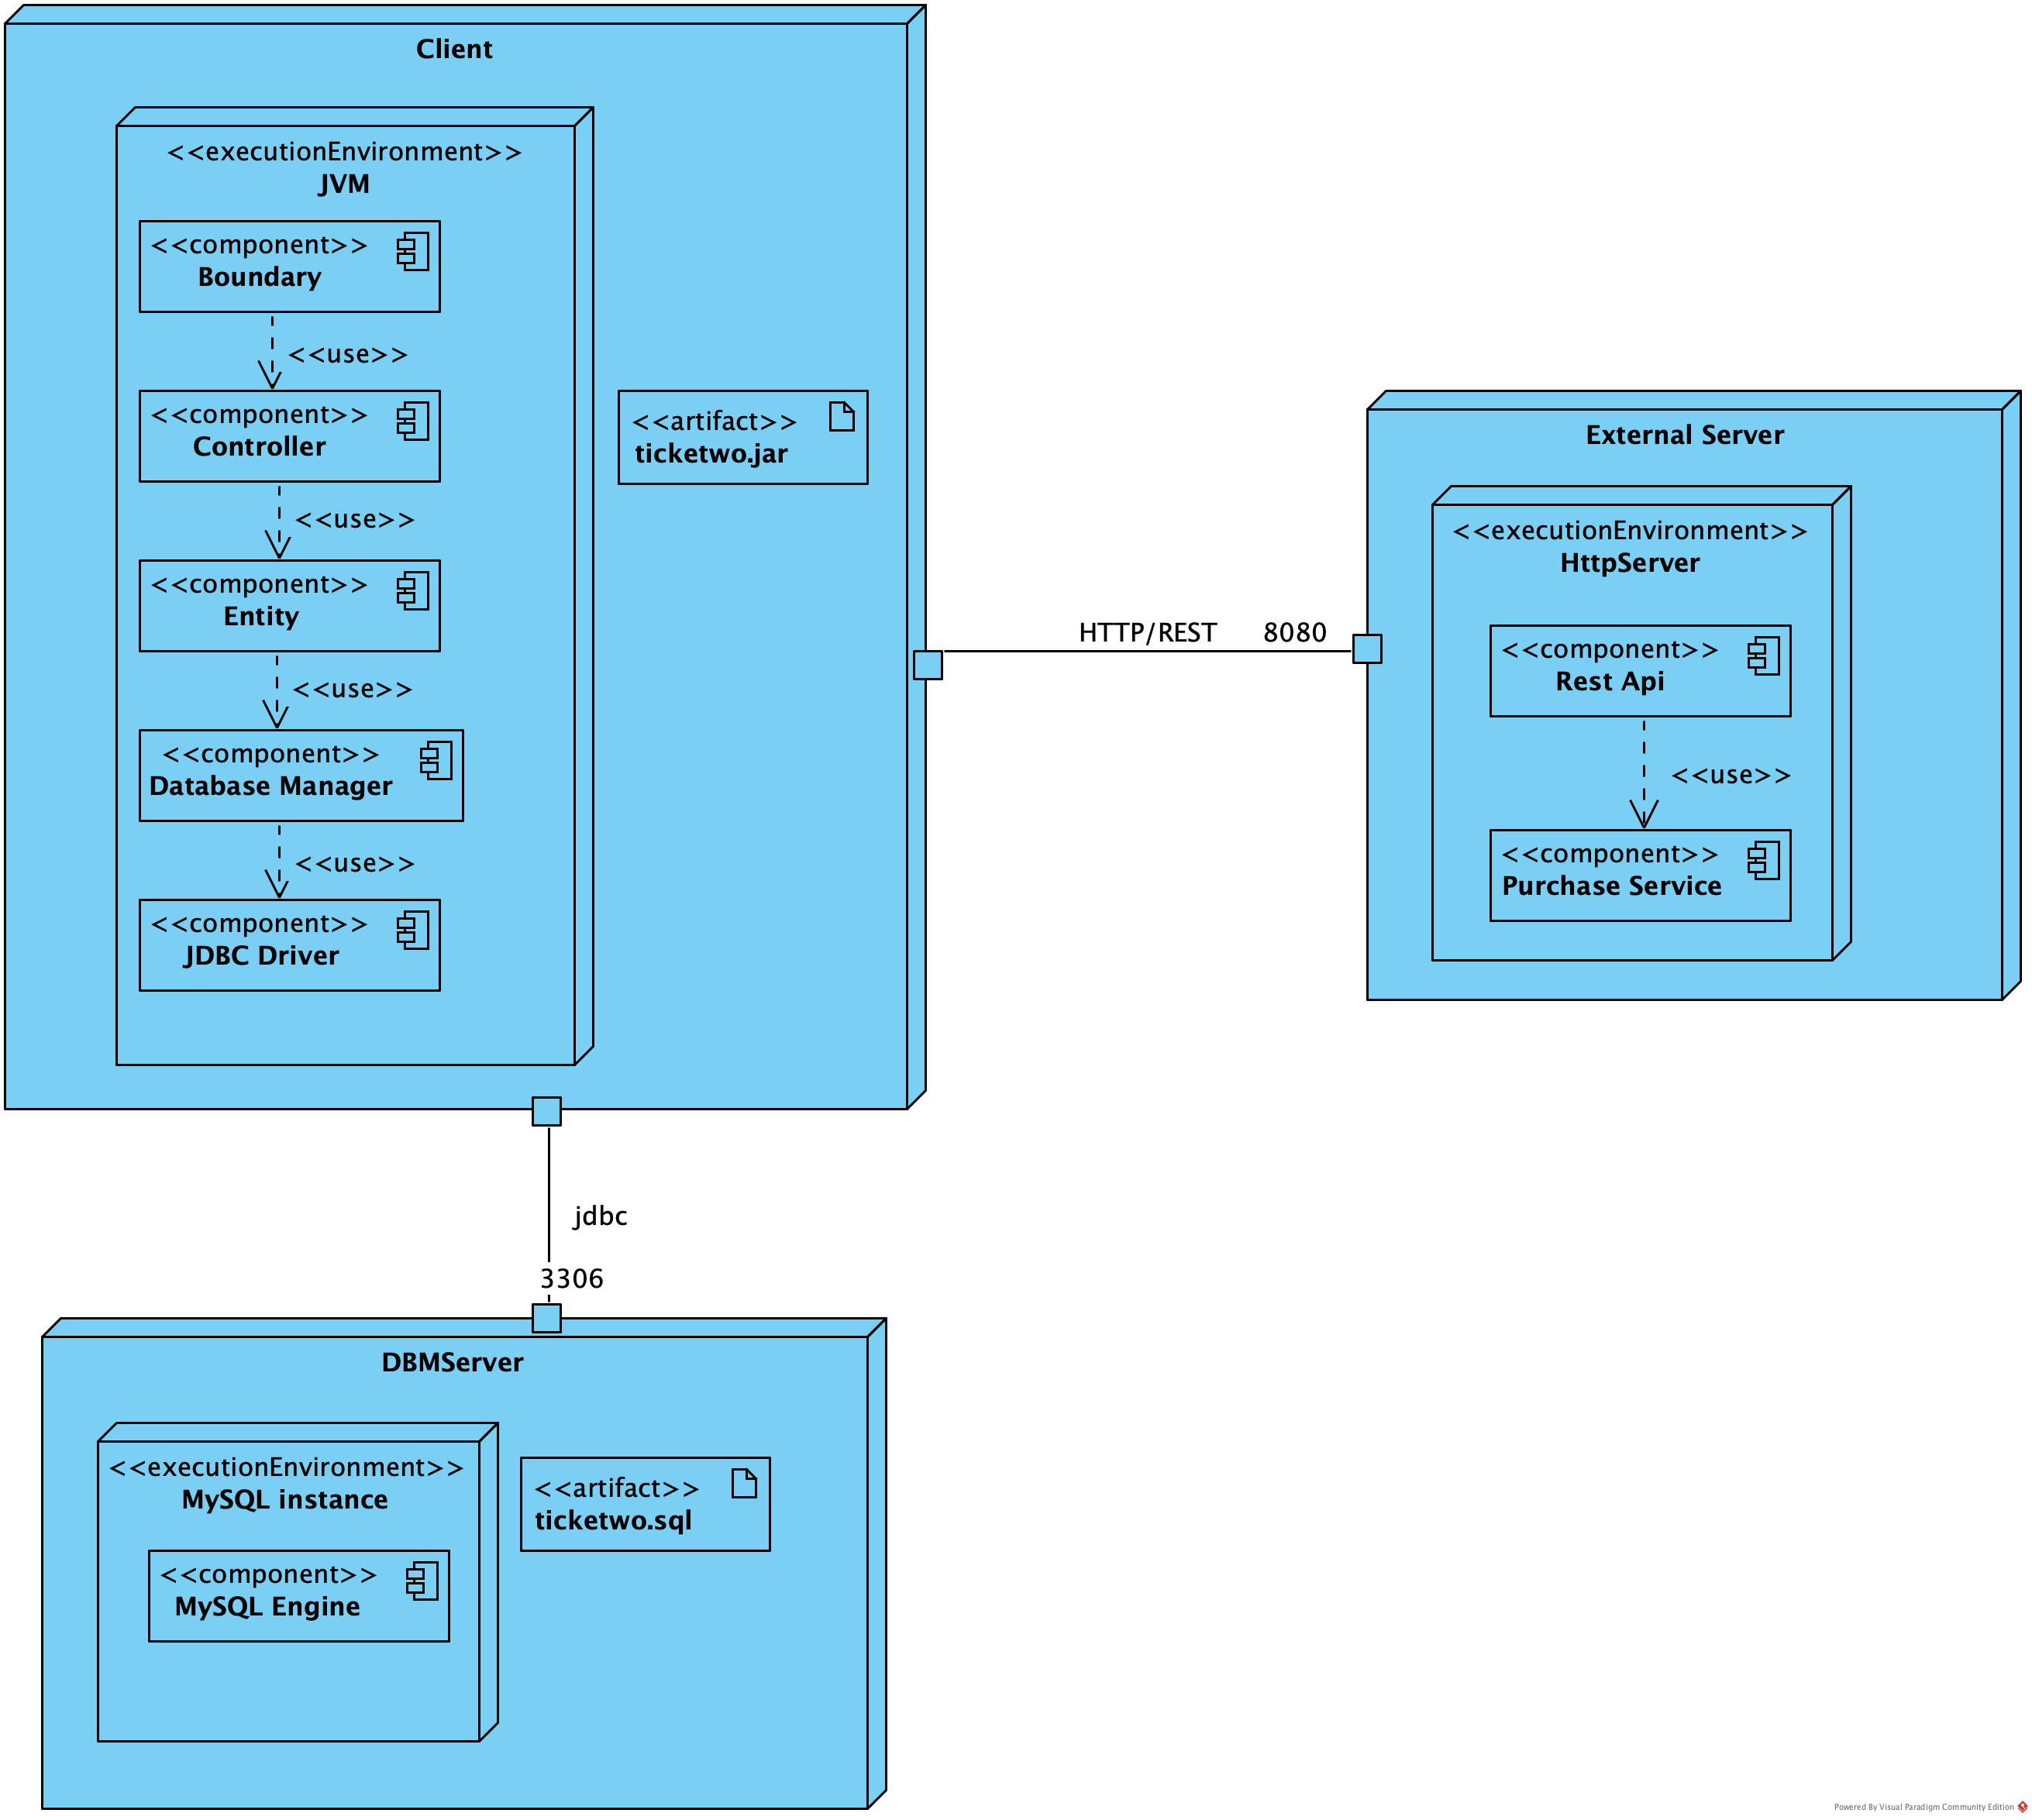
\includegraphics[width=0.5\linewidth]{assets/deployment/DeploymentDiagram}
\end{center}